\documentclass[
  journal=small,
  manuscript=mini-article,  % Use a - if you need a space e.g. "research-article"
  year=2026,
  volume=1,
]{odj-journal}

\usepackage{amsmath}
\usepackage[nopatch]{microtype}
\usepackage{booktabs}
\usepackage[square,sort,comma,numbers]{natbib}
\usepackage[colorlinks]{hyperref}
\hypersetup{
     colorlinks =true,
     linkcolor  =blue,
     filecolor  =blue,
     citecolor  =black,
     urlcolor   =cyan,
}
\usepackage{listings}
\usepackage{color}

\definecolor{dkgreen}{rgb}{0,0.6,0}
\definecolor{gray}{rgb}{0.5,0.5,0.5}
\definecolor{mauve}{rgb}{0.58,0,0.82}

\lstset{frame=tb,
  language=Python,
  aboveskip=3mm,
  belowskip=3mm,
  showstringspaces=false,
  columns=flexible,
  basicstyle={\small\ttfamily},
  numbers=none,
  numberstyle=\tiny\color{gray},
  keywordstyle=\color{blue},
  commentstyle=\color{dkgreen},
  stringstyle=\color{mauve},
  breaklines=true,
  breakatwhitespace=true,
  tabsize=3
}

\graphicspath{{../../figures/Gabri/}}

\title{Heat raises electricity demand in Catalonia more than cold does}

\author{Gabriel Albasini}
\affiliation{MSc in Physics of Complex Systems and Biophysics, Universitat de Barcelona, Barcelona, Spain.}
\email[Gabriel Albasini]{gabrielvalbasini@gmail.com}

\author{N\'uria Mayoral}
\affiliation{MSc in Physics of Complex Systems and Biophysics, Universitat de Barcelona, Barcelona, Spain.}

\author{Jes\'us Ruiz}
\affiliation{MSc in Physics of Complex Systems and Biophysics, Universitat de Barcelona, Barcelona, Spain.}

\author{Hug Sala}
\affiliation{MSc in Physics of Complex Systems and Biophysics, Universitat de Barcelona, Barcelona, Spain.}

\keywords{electricity demand; temperature; Catalonia; open data; piecewise linear regression}

\begin{document}

\begin{abstract}
Electricity demand depends on the weather, because buildings are heated on cold days and cooled on hot days. How strongly demand responds to heat compared with cold matters for planning the electricity system. Here we measure this response in Catalonia with open daily data for 912 working days of 2022--2025. We fitted a piecewise linear model of daily electricity demand against the mean temperature at an urban station in Barcelona. Demand is flat between 17 and 22\,$^\circ$C, at about 114\,GWh per day. Each degree below 17\,$^\circ$C adds 2.5\,\% of this base load, and each degree above 22\,$^\circ$C adds 3.7\,\%. Temperature explains 67\,\% of the daily variation, more than a seasonal curve based only on the date (52\,\%). Heat adds demand mainly in the afternoon, cold in the morning and in the evening. The same pattern appears with two other Barcelona stations. In Catalonia, warm weather therefore raises electricity use more per degree than cold weather.
\end{abstract}

\section{Background}

\textbf{Context.} In Spain, electricity demand responds to temperature in a non-linear way: it rises on cold days because of heating and on hot days because of cooling, with a minimum at mild temperatures \cite{valor2001,moral2005}. Threshold models, in which demand changes slope at one or more temperatures, describe this shape in several European countries \cite{bessec2008}. We ask two questions for Catalonia with recent open data: where is the comfort zone in which demand does not depend on temperature, and does one degree of heat add more or less demand than one degree of cold? Before the analysis we expected cold to weigh more, because heating is usually the main reason for high winter demand. This work is one part of a group project on climate extremes in Catalonia; the other parts study drought, crop yields and forest fires.

\textbf{Data.} Electricity demand comes from the dataset \emph{Demanda d'energia el\`ectrica hor\`aria a Catalunya per MWh}, published by the Catalan Energy Institute (ICAEN) on the Catalan open data portal \cite{icaen_demand}. It gives the hourly demand at power-station busbars, in MWh, for the network of the main electricity distributor in Catalonia, with one row per day (hourly columns and a daily total). It is updated monthly. Until September 2021 it also included energy passed on to other distributors, so we use data from 2022 onwards only, when the definition is constant. Temperature comes from the daily data of XEMA, the network of automatic weather stations of the Catalan Meteorological Service (Meteocat), published daily on the same portal \cite{xema}. We use the daily mean temperature (variable 1000) at station X4, Barcelona--el Raval (urban, 33\,m), and stations X8 (Zona Universit\`aria, 82\,m) and D5 (Observatori Fabra, 410\,m) as a check; station data come from the Meteocat station metadata \cite{xema_meta}. All data were downloaded through the portal's open API on 17 November 2026; no key is needed.

\section{Methods}

\textbf{Sample.} We joined demand and temperature by date (2,557 days, 2019--2025) and kept the weekdays from 2022 to 2025 that are not Catalan public holidays (998 days), using the \texttt{holidays} package \cite{holidays}. We removed August, the main holiday month, when demand is lower than expected for its temperature, and 28 April 2025, the day of the Iberian blackout (69\,GWh). The final sample has 912 days.

\textbf{Model.} Daily demand $D$ (GWh) is modelled as a function of the daily mean temperature $T$ with two thresholds:
\begin{equation}
D = \beta_0 + \beta_c \max(0,\, T_c - T) + \beta_h \max(0,\, T - T_h).
\label{eq:model}
\end{equation}
Below $T_c$ demand rises with slope $\beta_c$ per degree (cold), above $T_h$ with slope $\beta_h$ (heat), and between them it is constant at the base load $\beta_0$. For each pair of thresholds on a grid of 0.5\,$^\circ$C ($10 \le T_c \le 20$, $T_c \le T_h \le 24$) we found $\beta_0, \beta_c, \beta_h$ by least squares and kept the pair with the smallest residual sum of squares:
\begin{lstlisting}
def hinge_fit(t, y, t_cold, t_hot):
    X = np.column_stack([np.ones(len(t)),
                         np.clip(t_cold - t, 0, None),
                         np.clip(t - t_hot, 0, None)])
    coef, *_ = np.linalg.lstsq(X, y, rcond=None)
    return coef, ((y - X @ coef) ** 2).sum()
\end{lstlisting}
We report demand as a percentage of the base load, $100\,(D/\beta_0 - 1)$, so that the slopes read as \% per $^\circ$C.

\textbf{Comparison with a seasonal model.} Summer and winter also differ in daylight, activity and holidays. To test whether temperature explains demand better than the date itself, we fitted a seasonal model that uses only the day of the year (a mean plus two annual harmonics, least squares) and compared its coefficient of determination $R^2$ with that of Eq.~\eqref{eq:model} on the same 912 days. Both models have five free parameters (three coefficients and two thresholds, against five coefficients).

\textbf{Hour of the day.} The same dataset gives the demand of each hour (columns h01--h24, taken as hours 0--23). We dropped clock-change days and checked that the 24 hours add up to the daily total. Days were grouped into 2\,$^\circ$C bins of daily mean temperature, and the mean demand of each bin and hour was compared with the mean of mild days ($T_c \le T \le T_h$) at the same hour. Bins with fewer than 5 days are not shown.

\textbf{Other stations.} We repeated the fit with the temperature of stations X8 and D5 on the same days.

\textbf{Code and reproducibility.} All code is in the public repository \url{https://github.com/NuriaMayoral/XEMAS-}, in the notebook \texttt{gabri\_heat\_energy\_demand.ipynb} of the folder \texttt{notebook/}. The functions in \texttt{xema.py}, in the same folder, download each dataset through the API and save it as CSV in \texttt{data/raw/}, which is not versioned. To reproduce every number and figure: clone the repository, install the environment (\texttt{pip install -r requirements.txt holidays}) and run the notebook from the \texttt{notebook/} folder (\emph{Restart \& Run All}); the first run downloads the data. The analysis uses pandas, NumPy and Matplotlib \cite{pandas,numpy,matplotlib}.

\section{Results}

Figure~\ref{fig:temp} shows the daily demand against temperature. Demand is flat between $T_c = 17$\,$^\circ$C and $T_h = 22$\,$^\circ$C, with a base load $\beta_0 = 114.4$\,GWh per day. Below 17\,$^\circ$C demand rises by $\beta_c = 2.91$\,GWh (2.5\,\%) per degree; above 22\,$^\circ$C it rises by $\beta_h = 4.23$\,GWh (3.7\,\%) per degree. One degree of heat therefore adds more demand than one degree of cold. The residual scatter is large (root mean square error 5.8\,GWh): at the same temperature, winter days use more electricity than spring days, so temperature does not explain all the variation.

\begin{figure}[hbt!]
\centering
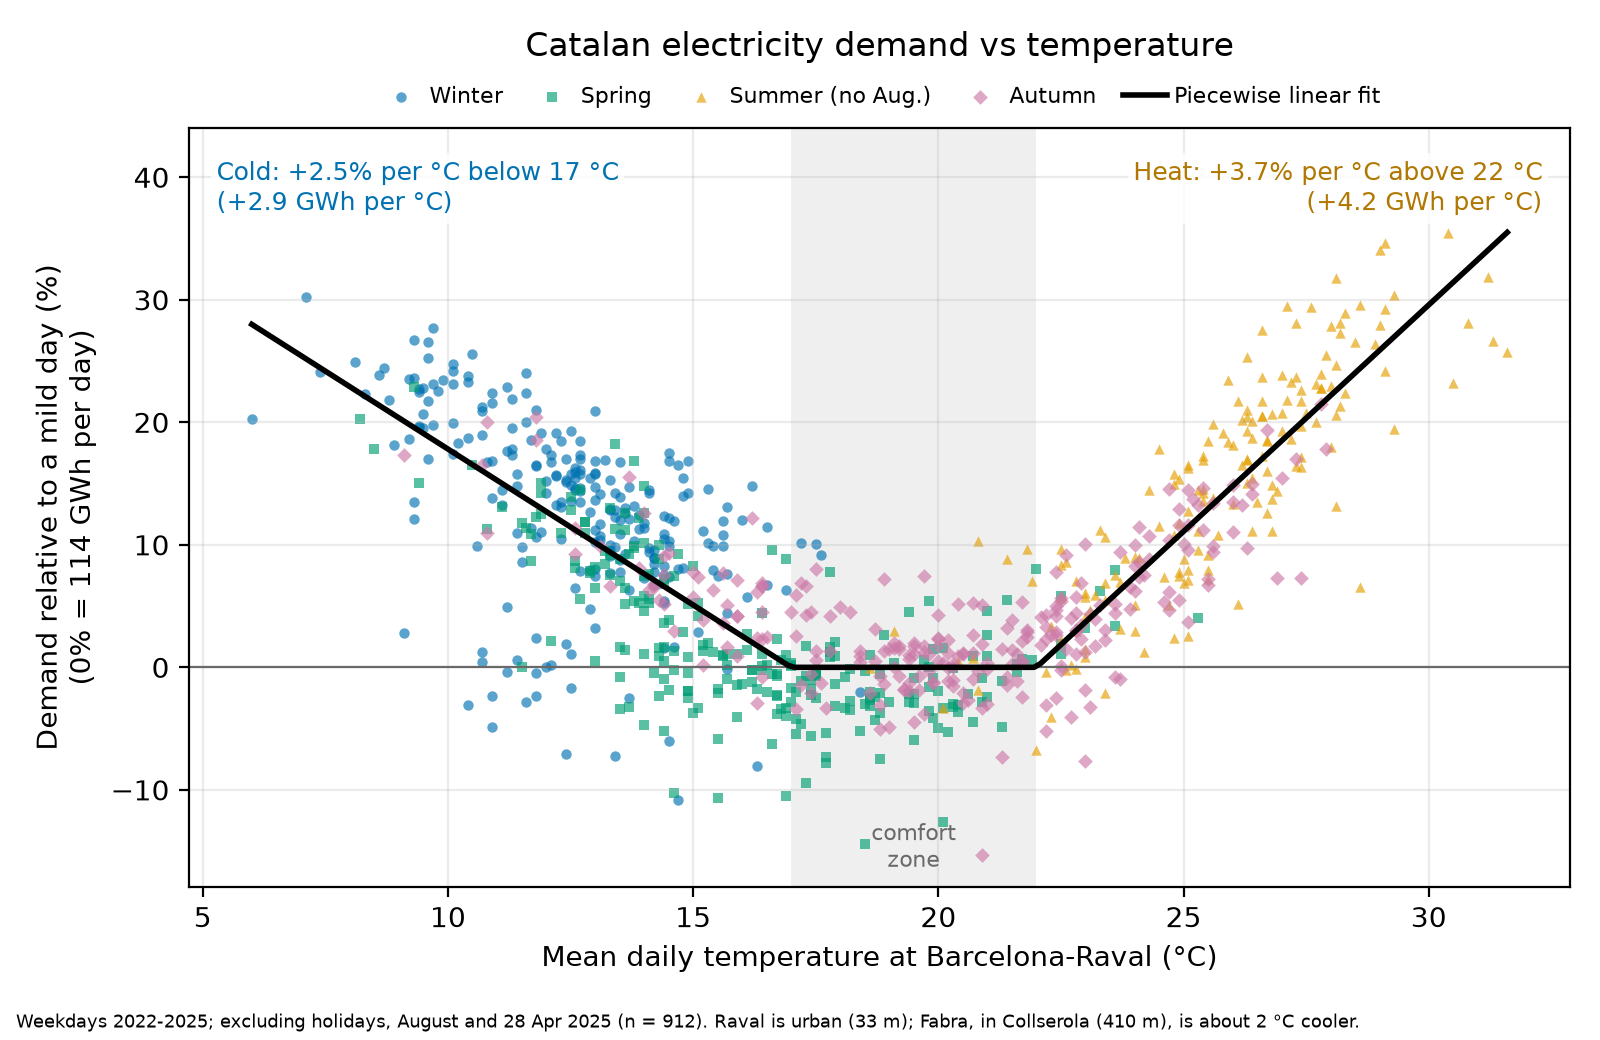
\includegraphics[width=\linewidth]{energy_demand_vs_temperature.png}
\caption{\textbf{Electricity demand in Catalonia is flat between 17 and 22\,$^\circ$C and rises faster with heat than with cold.} Daily demand on 912 weekdays of 2022--2025 (excluding public holidays, August and 28 April 2025) against the daily mean temperature at Barcelona--el Raval, as a percentage of the fitted base load (0\,\% = 114\,GWh per day). Colours and markers show the season. Black line: piecewise linear fit of Eq.~\eqref{eq:model}, with thresholds chosen by least squares on a 0.5\,$^\circ$C grid. Data: ICAEN \cite{icaen_demand}, Meteocat \cite{xema}.}
\label{fig:temp}
\end{figure}

Temperature explains more of the daily variation than the calendar. The seasonal model based on the date alone gives $R^2 = 0.52$, and the temperature model of Eq.~\eqref{eq:model} gives $R^2 = 0.67$, with the same number of parameters. On the same date, hot and cold days use more electricity than mild days, which the seasonal curve cannot capture.

Heat and cold add demand at different hours (Fig.~\ref{fig:hour}). On days of 28--30\,$^\circ$C, demand between 13 and 17\,h is 31--34\,\% higher than on mild days at the same hour, and 36--40\,\% higher on days of 30--32\,$^\circ$C (6 days). Hot days also keep demand high at night. On cold days (8--10\,$^\circ$C), the extra demand is largest in the morning (8--11\,h) and in the evening (18--20\,h), at 24--26\,\%.

\begin{figure}[hbt!]
\centering
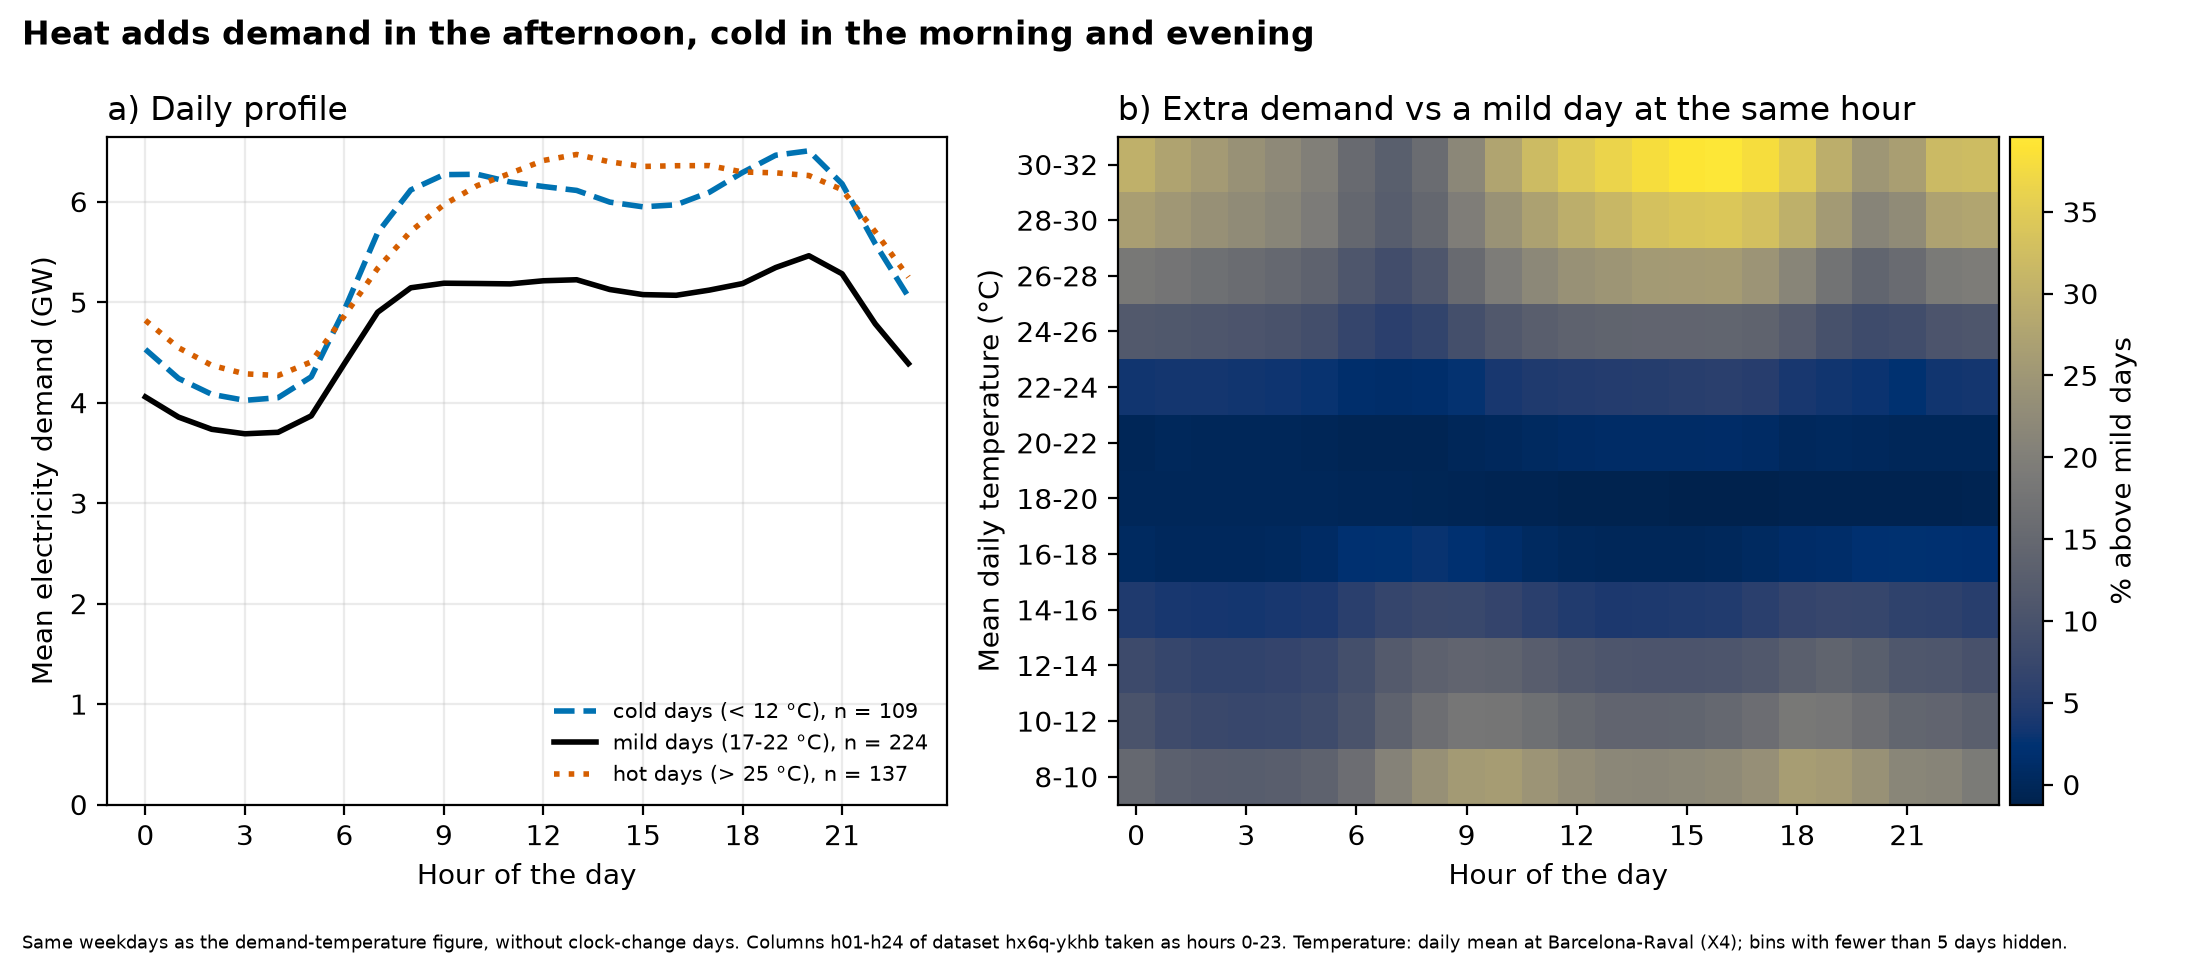
\includegraphics[width=\linewidth]{energy_demand_by_hour.png}
\caption{\textbf{Heat adds demand in the afternoon, cold in the morning and evening.} (a) Mean hourly demand on cold ($<12$\,$^\circ$C), mild (17--22\,$^\circ$C) and hot ($>25$\,$^\circ$C) days. (b) Extra demand at each hour, by 2\,$^\circ$C bin of daily mean temperature, as \% above mild days at the same hour; bins with fewer than 5 days are hidden. Same weekdays as Fig.~\ref{fig:temp}, without clock-change days.}
\label{fig:hour}
\end{figure}

The result does not depend on the station in its main features (Table~\ref{tab:stations}). With all three stations the heat slope is larger than the cold slope. The thresholds of the two urban stations are similar, while Fabra, on a forested hill and about 2\,$^\circ$C cooler, gives lower thresholds (15 and 19\,$^\circ$C) and fits slightly worse.

\begin{table}[hbt!]
\begin{threeparttable}
\caption{Fit of Eq.~\eqref{eq:model} with three Barcelona stations on the same 912 days.}
\label{tab:stations}
\begin{tabular}{lrrrrr}
\toprule
\headrow Station & Altitude & $T_c$ / $T_h$ & $\beta_c$ & $\beta_h$ & RMSE\\
\midrule
X4 el Raval (used) & 33\,m & 17 / 22\,$^\circ$C & 2.91 & 4.23 & 5.80\\
X8 Zona Universit\`aria & 82\,m & 17 / 21\,$^\circ$C & 2.54 & 3.90 & 5.76\\
D5 Observatori Fabra & 410\,m & 15 / 19\,$^\circ$C & 2.42 & 3.22 & 6.20\\
\bottomrule
\end{tabular}
\begin{tablenotes}[hang]
\item[]Slopes in GWh per $^\circ$C; RMSE (root mean square error of the fit) in GWh.
\end{tablenotes}
\end{threeparttable}
\end{table}

\section{Conclusions / Discussion}

In Catalonia, one degree of heat adds more electricity demand than one degree of cold: 3.7\,\% against 2.5\,\% of a mild day's demand per degree, outside a comfort zone of 17--22\,$^\circ$C. This was the opposite of our expectation. The pattern holds at three stations, and temperature explains the seasonal cycle of demand better than the calendar. The hourly profiles are consistent with air conditioning on hot afternoons and with heating in the morning and evening, although we did not test this. For the electricity system, this means that hot afternoons should be considered as well as cold winter evenings.

\textbf{Limitations.} We used one urban station for the temperature of all of Catalonia, while demand is regional. We used four years of weekdays only, excluded August, and evaluated the fit in-sample, without cross-validation. The demand dataset covers the main distributor's network, not all of Catalonia. The model includes neither prices, economic activity nor daylight, so the slopes describe an association, not a causal effect. The daily mean temperature cannot resolve the hourly response, and the hour convention of the dataset (h01 as 00--01\,h) is assumed, not documented.

\textbf{Future work.} The next step would be to use hourly temperature from several stations, weighted by the population or the demand of each area, and test the model on a year left out of the fit. Data on air-conditioning ownership, electricity prices and the demand of all distributors would allow us to separate the effect of temperature from other drivers, and to see whether the heat slope grows over time.

\bibliographystyle{acm}
\bibliography{gabri_refs}

\end{document}
